% Configure pgfplots to interpret commas as decimal points
\pgfplotsset{
    every axis/.append style={
        tick label style={/pgf/number format/use comma, /pgf/number format/1000 sep={}}
    }
}

\begin{figure}[h!]
\centering
\caption{Balance (déficit o superávit) del GNC}
\label{fig:Balance}
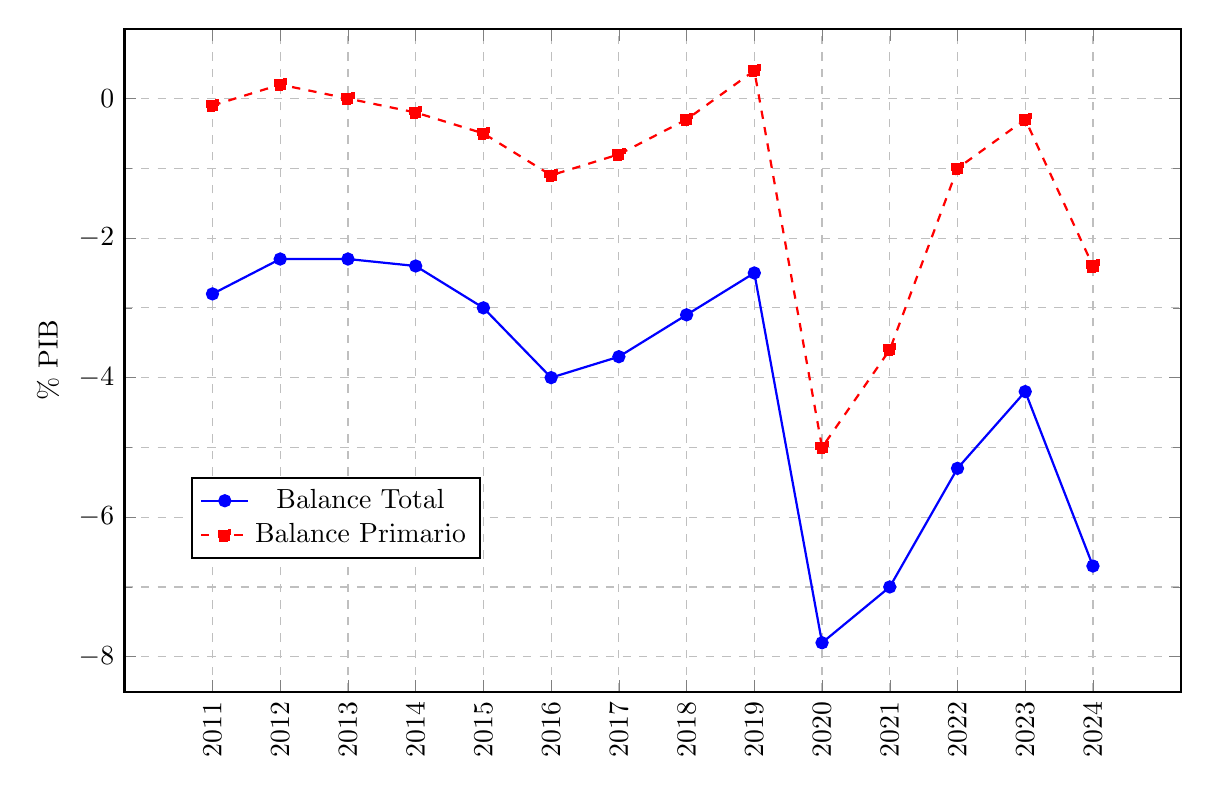
\begin{tikzpicture}
\begin{axis}[
    width=15cm,
    height=10cm,
%    xlabel={Años},
    ylabel={\% PIB},
    xtick=data,
    xticklabels={
    %    {2004}, {2005}, {2006}, {2007}, {2008}, {2009}, {2010}, 
    {2011}, {2012}, {2013},
        {2014}, {2015}, {2016}, {2017}, {2018}, {2019}, {2020}, {2021}, {2022}, {2023}, {2024}
    },
    x tick label style={rotate=90, anchor=east},
    ymin=-8.5,
    ymax=1,
    ymajorgrids=true,
    grid style=dashed,
    grid = both,
    grid=major,
    grid=both,
    grid style=dashed,
    minor y tick num=1,
    legend style={at={(0.2,0.2)}, anchor=south},
    thick]

% Datos del Balance Total
\addplot[
    color=blue,
    mark=*,
    solid
] coordinates {
% (0,-4.5)	(1,-4.0)	(2,-3.4)	(3,-2.7)	(4,-2.3)	(5,-4.1)	(6,-3.9)
(7,-2.8) (8,-2.3) (9,-2.3) (10,-2.4) (11,-3.0) 
(12,-4.0) (13,-3.7) (14,-3.1) (15,-2.5) (16,-7.8) 
(17,-7.0) (18,-5.3) (19,-4.2) (20,-6.7)
};

% Datos del Balance Primario
\addplot[
    color=red,
    mark=square*,
    dashed
] coordinates {
%(0,-0.9)	(1,-0.9)	(2,0.2)	(3,1.0)	(4,0.9)	(5,-1.1)	(6,-1.1)	
(7,-0.1)	(8,0.2)	(9,0.0)	(10,-0.2)	(11,-0.5)	(12,-1.1)	(13,-0.8)	(14,-0.3)	(15,0.4)	(16,-5.0)	(17,-3.6)	(18,-1.0)	(19,-0.3) (20,-2.4)
};
\legend{Balance Total, Balance Primario}
\end{axis}
\end{tikzpicture}
\par \footnotesize{\textit{Fuente: \textcite{minhacienda_balance_2025}}}
\end{figure}
%%%%%%%%%%%%%%%%%%%%%%%%%%%%%%%%%%%%%%%%%%%%%%%%%%%%%%%%
%%%%%%%%%%%%%%%%%%%%%%%%%%%%%%%%%%%%%%%%%%%%%%%%%%%%%%%%
